\documentclass[12pt]{article}

\usepackage[english]{babel}
\usepackage[utf8x]{inputenc}
\usepackage{pdfpages}
\usepackage{lastpage} % Required to determine the last page for the footer
\usepackage{extramarks} % Required for headers and footers
\usepackage{graphicx} % Required to insert images
\usepackage{listings} % Required for insertion of code
\usepackage{courier} % Required for the courier font
\usepackage{color}
\usepackage{grffile}
\usepackage{float}

\usepackage[a4paper, total={6in, 8in}]{geometry}

% Margins
\topmargin=-0.45in
\evensidemargin=0in
\oddsidemargin=0in
\textwidth=6.5in
\textheight=9.0in
\headsep=0.25in
\fboxsep=0mm%padding thickness
\fboxrule=2pt%border thickness

\linespread{1.1} % Line spacing

\newcommand{\Title}{Architecture specification Document} % Assignment title
\newcommand{\Class}{Cos\ 301} % Course/class
\newcommand{\pd}{Post-Doctoral}
\newcommand{\ssr}{Soft\color{green}{Serve }\color{black}}
\newcommand{\version}{1.0}
\newcommand{\iteration}{1}
\newcommand{\client}{Ms. Cathy Sandis (UP Research Office)}
\newcommand{\project}{Post-Doctoral Application Management System}
\newcommand{\repo}{https://github.com/mox1990/Project-Postdoc.git}

\begin{document}


\vspace{4em}

\begin{center}%

\begin{figure}[ht!]
\centering

\includegraphics{../Images_Docs/logo.png}
\end{figure}
\LARGE \bf \project \\[1em]
\LARGE \bf \Title \\[0.25em]
\large \bf \today\\
\bf Version \version\\
\bf Iteration \iteration\\[0.5em]
\Large \bf Prepared for \client\\
\Large \bf by
\Large {\bf \ssr Group }\\[0.5em]
\LARGE {\bf Group members}\\[0.25em]
\large
Kgothatso Phatedi Alfred Ngako (12236731) \\[0.5em]
Tokologo “Carlo” Machaba (12078027) \\[0.5em]
Mathys Ellis (12019837) \\[8em]

\end{center}%

%\newpage
%{\LARGE \bf Change log}\\[2em]

\begin{center}
\begin{tabular}{|l|p{1.4cm}|p{8cm}|p{2.8cm}|}
\hline
\multicolumn{4}{|c|}{\bf Change log} \\
\hline
 Date & Version & Description &  Person \\
\hline
18/05/2014 & v 0.0 & Document created. & Alfred Ngako \\
\hline
19/05/2014 & v 0.1 & Added more detail to information in subsections. & Alfred Ngako \\
\hline
20/05/2014 & v 0.2 & Added references and citations. & Alfred Ngako \\
\hline
22/05/2014 & v 0.3 & Transferred architectural scope to architectural requirements specification document. Began editing. & Mathys Ellis \\
\hline
23/05/2014 & v 0.4 & Added to and edited architectural patterns and style. & Mathys Ellis \\
\hline
%\end{tabbing}
\end{tabular}
\end{center}
\newpage
\tableofcontents

\listoffigures
\newpage
\section{Project Repository}
\textbf{\repo}
\newpage
%%%%%%%%%%%%%%%%%%%%%%%%%%%%%%%%%%%%%%%%%%%%%%%%%%%%%%%%%%%%%%%%%%%%%%%%%%%%%%%%%%%%%%%%%%%%%%%%%%%%%%%%%%%%%

\section{Document description:}%Not entirely sure what I should add here

\subsection{Document purpose}
\vspace{0.2in}

This document follows on the Architecture requirements specification document. The Architecture specification document provides the architectural descriptions of various architectural factors that the project will need to follow when developing the system.  Architecture in this document's context refer to the technological basis and software development styles of the project. Thus this document serves as a contract between SoftServe and the client, Mrs Cathy Sandis of the DRIS of the University of Pretoria in terms of what technologies the project should incorporate as-well the software development infrastructure that the system will be based on.
\vspace{0.2in}

\subsection{Documentation methodology}
\vspace{0.2in}
\begin{flushleft}
The documentation and software development methodology used by the project adhere to the guidelines set out by the scum agile methodology. Thus this document has undergone and will undergo various iterations that may extend or reduce the contents of the document.\\

The document was compiled using a software architecture specification document template provided by Dr Fritz Solms as an alternative to the Kruchten 4 + 1 approach to documenting software.

This document was created using the requirement elicitation techniques and requirement definitions as specified by Klaus Pohl’s book Requirements Engineering: Fundamentals, Principles, and Techniques [Dr.Phol, K., 2010].
The requirements, vision and scope were elicited from the following sources:
\begin{itemize}
	\item Numerous interviews with the client.
	\item On-line research into UP Post doctoral applications.
	\item Correspondence with the UP IT department.
	\item Collecting and analysing various documents such as:
		\begin{itemize}
			\item The initial project request document
			\item Application forms
			\item Renewal forms
			\item CV templates
			\item Approval and recommendation forms
		\end{itemize}
\end{itemize}
\end{flushleft}	

\vspace{0.5in}

\subsection{Document conventions:}
\vspace{0.1in}
\begin{itemize}
\item Documentation formulation tool: LaTeX
\end{itemize}

\vspace{0.2in}

\subsection{References:}
\vspace{0.1in}
\begin{itemize}
\item Kang, A. August 9, 2002, \textit{Enterprise application integration using J2EE}, Available from: http://www.javaworld.com/article/2074488/enterprise-java/enterprise-application-integration-using-j2ee.html , [Accessed on: 17 May 2014]
\item Ali Babar, M., \textit{Architectural Patterns and Frameworks, Week 3, Lecture 3},Available from: https://blog.itu.dk/MSAR-E2013/files/2013/09/wk3\_lect3\_patternsframeworktactics.pdf, [Accessed on: 21 May 2014]
\item Dr.Phol, K., 2010, \textit{Requirements Engineering: Fundamentals, Principles, and Techniques}, Springer, Heidelberg.
\item Kayal, D., 2008, \textit{Pro Java EE Spring Patterns: Best Practices and Design Strategies Implementing Java EE patterns with Spring Framework}, Apress, New York.
\item Jendrock E, Cervera-Navarro R, Evans I, Haase K, Markito W, \textit{The Java EE 7 Tutorial}, Available from: http://docs.oracle.com/javaee/7/tutorial/doc/home.htm , [Accessed on: 20 May 2014]
\item Oracle. April 2014, \textit{The Java EE 7 Tutorial}, Available from: http://docs.oracle.com/javaee/7/tutorial/doc/overview.htm , [Accessed on: 20 May 2014]
\end{itemize}	

\vspace{0.5in}

\newpage

%%%%%%%%%%%%%%%%%%%%%%%%%%%%%%%%%%%%%%%%%%%%%%%%%%%%%%%%%%%%%%%%%%%%%%%%%%%%%%%%%%%%%%%%%%%%%%%%%%%%%%%%%%%%%
\section{Architecture Requirements} 
This section can be found in the architecture requirements specification document in which it discusses the following:
\begin{itemize}
\item Architectural scope
\item Access channel requirements
\item Quality Requirements
\item Integration requirements
\item Architectural Constraints
\end{itemize}

%%%%%%%%%%%%%%%%%%%%%%%%%%%%%%%%%%%%%%%%%%%%%%%%%%%%%%%%%%%%%%%%%%%%%%%%%%%%%%%%%%%%%%%%%%%%%%%%%%%%%%%%%%%%%


\section{Architectural Patterns and Styles} % skipped till further notice.

% Mention of how Java EE actually doesn't require use of GoF design patterns >> http://www.theserverside.com/tip/With-Java-EE-7-your-Design-Patterns-are-dead-And-your-EAR-is-ugly-too <<

The system will employ the Model-View-Controller, MVC, architectural pattern combined with a multi-tier/layered architectural pattern to form what is known as the Java Enterprise Edition system architecture. This will allow the client(s) to be decoupled from the server. Further this allows the view, the controller and the model each to have its own set of layers. Both of these patterns provide various benefits and are widely used. Some benefits include modularity, encapsulation, re-usability of components, decoupling and system maintainability [Ali Babar, M.] [Oracle, 2014][Kayal, D., 2008]\\
\\
The Java EE system architecture is designed to support highly scalable, distributed, transactional, and portable applications that use the speed, security, and reliability of a Java EE server to provide powerful enterprise applications. [Oracle, 2014] For this reason SoftServe believes this system architecture is well suited for the development of the Post-Doctoral application management system as it will satisfy the requirements in terms of quality and functional as stipulated by the client. The following diagram provides the system architectural that will be employed by the system:\\

\begin{figure}[H]
\centering
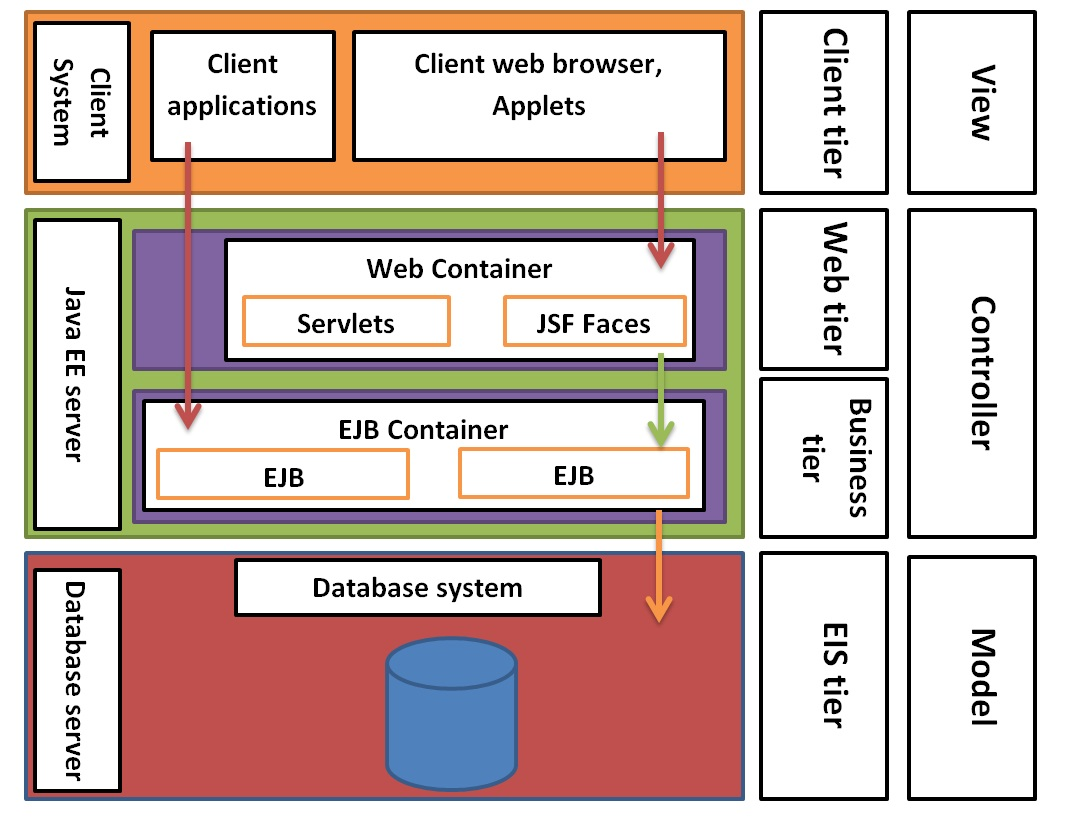
\includegraphics[scale=0.8]{../Images_Docs/Diagrams/Architecture/Java EE system architecture.jpg}
\caption{Java EE system architecture}
\end{figure}

\subsection{View}
The View component of the system architecture is used to represent and encapsulate the front-end of the system. It contains the client tier of the Java EE system architecture. Thus this allows the system to decouple the front-end and the back-end components. Allowing various clients to access the back-end without having to duplicate certain back-end tiers for each client. [Kayal, D., 2008]
\subsubsection{Client Tier}
This tier runs on the client system and encapsulates the various components that a client system may use to access the Java EE server-side tiers. These components include dynamic web pages, Java applications and Java applets. In order to make the Post-doctoral application management system accessible to any stakeholder over the internet and provide a uniform user experience the system will only make use of the dynamic web pages component provided by the Java EE client tier. [Oracle, 2014]  
\subsection{Controller}
The controller component of the system architecture is used to provide the business logic and manage and manipulate the view's request in order to provide communication between the Model component and the View. This component therefore hosts the web tier and the business tier of the Java EE application. This component is located on the Java EE server which is a multi-threaded application server. [Kayal, D., 2008] [Oracle, 2014] 
\subsubsection{Web Tier}
This Tier runs on the Java EE server and hosts the Web container. It provides the management and web page generation support for the web pages that the system has to provide to the view through the user of servlets, Java ServerPages and Java ServerFaces Facelets. Facilitates the communication between the business tier and client tier for web browser clients and applets. Client applications do not have to make use of the Web Tier and can directly skip to the business tier. But as stipulated above the other types of client components will not be considered for the project. [Oracle, 2014]
\subsubsection{Business Tier}
This Tier also runs on the Java EE server and hosts the Enterprise Java Bean container. It provides the business logic section for the Java EE application in the form of Enterprise Java Beans which are simply classes that represent various persistence entities of the data base, system messages, sessions, etc. This tier communicates with EIS tier in order to get access the database and various other lower level infrastructures that the Java EE application requires. [Oracle, 2014]
% More bullshit goes here.
\subsection{Model}
The Model component of the system architecture contains the various persistence storage infrastructure and lower level system management features such as transaction processing. It hosts the Enterprise Information System tier of the Java EE application. [Kayal, D., 2008]
\subsubsection{Enterprise Information Tier} 
The EIS tier provides mainly the support for database systems that is used by the Java-EE application. This tier can run on the Java-EE server as a virtual server or on a physically different database server. Due to the project budget and technical constraints the former will used by the system. [Oracle, 2014] 
 
%%%%%%%%%%%%%%%%%%%%%%%%%%%%%%%%%%%%%%%%%%%%%%%%%%%%%%%%%%%%%%%%%%%%%%%%%%%%%%%%%%%%%%%%%%%%%%%%%%%%%%%%%%%%%
\section{Architectural Tactics and Strategies} % skipped till further notice.
This section describes techniques which will be used to satisfy the quality requirements. 

% This section needs a lot of paraphrasing...
\subsection{Concurrency}
The Java Platform has always offered support for concurrent programming, which is the basis for implementing many of the services offered by Java EE containers. This is realized through the two main concepts of having a multiple threads execute under a single process, in the case of Java EE mulitple beans execute under the JVM. The number of threads that can execute under the JVM can go well beyond thousands depending on factors such as the machine the JVM is running on and how it has been configured.\\

Even though the concurrent threads will mean better performance and a scalable implementation for the system they may lead to issues that effect the reliability and integrity of the system such as:
\begin{itemize}
\item Deadlocks,
\item Thread Starvation,
\item Concurrent  accessing of shared resources, and
\item Situations where the program generates incorrect data.
\end{itemize}

To deal with these issues Java EE provides concurrent utilities that access concurrent resources via JNDI lookup or resource injection. The components in the utilities ensure that the issues mentioned above are nullified. The primary components of interest in the concurrent utilities for our system are:
\begin{itemize}
\item managed executor service, 
\item managed scheduled executor service, 
\item managed thread factory, and 
\item context service.
\end{itemize}

\subsubsection{Managed Executor Service}
A managed executor service is used by applications to execute submitted tasks asynchronously. Tasks are executed on threads that are
started and managed by the container. The context of the container is propagated to the thread executing the task.

For example, by using an ManagedExecutorService.submit() call, a task, such as the GenerateReportTask, could be submitted to execute at a later time and then, by using the Future object callback, retrieve the result when it becomes available ().

\subsubsection{Managed Scheduled Executor Service}
A managed scheduled executor service is used by applications to execute submitted tasks asynchronously at specific times. Tasks are executed on threads that are started and managed by the container. The context of the container is propagated to the thread executing the task. The API
provides the scheduling functionality that allows users to set a specific date/time for the Task execution programmatically in the application.

\subsubsection{Managed Thread Factory}
A managed thread factory is used by applications to create managed threads. The threads are started and managed by the container. The context of the container is propagated to the thread executing the task. This object can also be used to provide custom factories for specific use cases (with custom Threads) and, for example, set specific/proprietary properties to these objects (Cervera-Navarro, Evans, Jendrock, Haase and Markito 2014).


%%%%%%%%%%%%%%%%%%%%%%%%%%%%%%%%%%%%%%%%%%%%%%%%%%%%%%%%%%%%%%%%%%%%%%%%%%%%%%%%%%%%%%%%%%%%%%%%%%%%%%%%%%%%%
\section{Use of Reference Architecture and Framework}
Java EE provides an API and runtime environment for developing and running large-scale, multi-tiered, scalable, reliable, and secure network applications. It also provides an architecture for implementing services as multitier applications that deliver the scalability, accessibility, and manageability needed by the system. This is reason to why it is ideal to use it in the development of the project.

It allows easy development of thin-client multi tiried applications without the many lines of complicated code that handles transactions or state management. Business logic is organized into reuseable components and provides underlying services as containers for all component types.

The features in the JavaServer Faces technology provided HTML5 friendly markup which will assist in the implementation of the user friendly UI.

\subsection{Java Persistence}
Java EE is in itself implemented as a object oriented model, yet it is expected to function with mainly relational databases. To bridge the gap between an object-oriented model and a relational database an object/relational mapping approach will be used to achieve Persistence. Java Persistence consists of the following areas:
\begin{itemize}
\item The Java Persistence API,
\item The query language, and
\item Object/relational mapping metadata
\end{itemize}

\subsection{RESTful web services}
RESTful web services are loosely coupled, lightweight web services that are particularly well suited for creating APIs for clients spread out across the internet. Representational State Transfer (REST) is an architectural style of client-server application centered around the transfer of representations of resources through requests and responses. In the REST architectural style, data and functionality are considered resources and are accessed using Uniform Resource Identifiers (URIs), typically links on the Web. The resources are represented by documents and are acted upon by using a set of simple, well-defined operations.

In Java EE 7, JAX-RS provides the functionality for Representational State Transfer (RESTful) web services. JAX-RS is a Java programming language API designed to make it easy to develop applications that use the REST architecture.

The JAX-RS API uses Java programming language annotations to simplify the development of RESTful web services. Developers decorate Java programming language class files with JAX-RS annotations to define resources and the actions that can be performed on those resources. JAX-RS annotations are runtime annotations; therefore, runtime reflection will generate the helper classes and artifacts for the resource. A Java EE application archive containing JAX-RS resource classes will have the resources configured, the helper classes and artifacts generated, and the resource exposed to clients by deploying the archive to a Java EE server (Cervera-Navarro, Evans, Jendrock, Haase and Markito 2014).

%%%%%%%%%%%%%%%%%%%%%%%%%%%%%%%%%%%%%%%%%%%%%%%%%%%%%%%%%%%%%%%%%%%%%%%%%%%%%%%%%%%%%%%%%%%%%%%%%%%%%%%%%%%%%
\section{Access and Integration channels}
This section discusses the requirements for the channels through which the system can be accessed by humans and other systems. Also making mention about the integration channels which need to be followed. 

\subsection{Access Channels}
The system will be accessible by humans through the recent versions of the following browsers:
\begin{enumerate}
\item Mozilla Firefox 20+
\item Google Chrome 30+
\item Microsoft Internet Explorer 9+
\item Apple Safari
\item Opera
\end{enumerate}
The mobile counterparts of the above mentioned browsers will also be catered for and so no other access channel (such as Android/Apple apps) is to be considered.
\subsection{Integration Channels}
Upon successful complementation the system must be integratedable with the University of Pretoria's PeopleSoft system. Therefore it is sensible to implement the system in Java EE as it is one of the many components that form part of the multiple tiers that build up  PeopleSoft. \\
\\
The use of build tools such as Maven will provide a central piece of information with regards to the projects build, reporting and documentation. This central point of information will assist in the integration phase since it is implemented through a standardised build approach which can come into play at a later time through the use of EAI.\\
\\
The EAI will be achieved via  the logical integration architecture of Direct point-to-point integration (Kang, 2002). This means that the application management system will make direct JDBC calls to the universities databases tables (which needed to be setup to cater for our system at that point). The Integration method will be pushed-based data-level integration (or if all else fails UI-Level integration).
% http://www.javaworld.com/article/2074488/enterprise-java/enterprise-application-integration-using-j2ee.html

\section{Technologies}
The System will use the following technologies:
\begin{itemize}
\item Java Enterprise Edition 7, 
\item MySQL database, open-source relational database management system
\item Netbeans 8.0
\item Glassfish server
\end{itemize}

\subsection*{Integrated Development Environment}
The system should be buildable independent of an IDE but it will be developed on Netbeans 8.0 to allow for uniformity amongst the development team, with regards to coding style, and provide easy integration with the tools that will be used such as Javadoc, to generate  API documentation in HTML format.

\subsection*{API}
\begin{itemize}
\item Java Persistence API. The Java Persistence API (JPA) is a Java standards–based solution for persistence.
\item JavaMail. API used to send email notifications.
\item JavaBeans Activation Framework. The JavaBeans Activation Framework (JAF) is used by the JavaMail API. JAF provides standard services to determine the type of an arbitrary piece of data, encapsulate access to it, discover the operations available on it, and create the appropriate JavaBeans component to perform those operations.
\item Java Database Connectivity. The Java Database Connectivity (JDBC) API lets you invoke SQL commands from Java programming language methods. You use the JDBC API in an enterprise bean when you have a session bean access the database. You can also use the JDBC API from a servlet or a JSP page to access the database directly without going through an enterprise bean.
\item Java Naming and Directory Interface. The Java Naming and Directory Interface (JNDI) API provides naming and directory functionality, enabling applications to access multiple naming and directory services, such as LDAP, DNS, and NIS. The JNDI API provides applications with methods for performing standard directory operations, such as associating attributes with objects and searching for objects using their attributes. Using JNDI, a Java EE application can store and retrieve any type of named Java object, allowing Java EE applications to coexist with many legacy applications and systems.
\item Java API for XML Web Services. The Java API for XML Web Services (JAX-WS) specification provides support for web services that use the JAXB API for binding XML data to Java objects. The JAX-WS specification defines client APIs for accessing web services as well as techniques for implementing web service endpoints. The Implementing Enterprise Web Services specification describes the deployment of JAX-WS-based services and clients. The EJB and Java Servlet specifications also describe aspects of such deployment. JAX-WS-based applications can be deployed using any of these deployment models.
\item SOAP with Attachments API for Java. The SOAP with Attachments API for Java (SAAJ) is a low-level API on which JAX-WS depends. SAAJ enables the production and consumption of messages that conform to the SOAP 1.1 and 1.2 specifications and the SOAP with Attachments note.
\item Java Authentication and Authorization Service. The Java Authentication and Authorization Service (JAAS) provides a way for a Java EE application to authenticate and authorize a specific user or group of users to run it.
\end{itemize}

\subsection*{Build Tools}
\begin{itemize}
\item Apache Maven (for reasons explained in the integration channels section).
\end{itemize}

\subsection*{Operating System}
The system will be deployable on:
\begin{itemize}
\item Windows 7 and 8.
\item Linux based operating systems (specifically Kububuntu 13).
\end{itemize}
\newpage

\section{Glossary:} %Mathys
\vspace{0.2in}

\begin{itemize}

\item \textbf{API} - Application Programming Interface
\item \textbf{Application} -Both renewal applications or new fellowship applications are seen as applications by this project.
\item \textbf{CV} - Curriculum Vita
\item \textbf{EAI} - Enterprise Application Integration
\item \textbf{HTML} - Hyper Text Mark-up Language
\item \textbf{Java EE} - Java Enterprise Edition
\item \textbf{JDBC} - Java Database Connection
\item \textbf{MVC} - Model View Controller
\item \textbf{UI} - User Interface
\item \textbf{UP} - University of Pretoria
 
\end{itemize}	

\end{document}